%%
%% This is file `introb2026.tex',
%% ACM sigconf format for IntRob 2026.
%%
\documentclass[sigconf]{acmart}

\AtBeginDocument{%
  \providecommand\BibTeX{{%
    Bib\TeX}}}

\setcopyright{acmlicensed}
\copyrightyear{2026}
\acmYear{2026}
\acmDOI{10.1145/XXXXXXX.XXXXXXX}
\acmConference[IntRob'26]{Intelligent Robotics FAIR 2026}{June 2026}{Budapest, HU}
\acmISBN{978-1-4503-XXXX-X/2026/06}
\acmSubmissionID{10}

\usepackage{booktabs}
\usepackage{amsmath}
\usepackage{algorithm}
\usepackage{algorithmic}
\usepackage{graphicx}

\begin{document}

\title{Targeted Behavioral Unlearning for Discrete On-Policy Reinforcement Learning}

\author{Tam\'as Tak\'acs}
\authornote{Both authors contributed equally to this research.}
\email{tamastheactual@inf.elte.hu}
\orcid{0009-0006-3027-7491}
\affiliation{%
  \institution{ELTE E\"otv\"os Lor\'and University}
  \city{Budapest}
  \country{Hungary}
}

\author{L\'aszl\'o Guly\'as}
\authornotemark[1]
\email{lgulyas@inf.elte.hu}
\orcid{0000-0002-6367-6695}
\affiliation{%
  \institution{ELTE E\"otv\"os Lor\'and University}
  \city{Budapest}
  \country{Hungary}
}

\renewcommand{\shortauthors}{Tak\'acs and Guly\'as}

\begin{abstract}
Machine unlearning in reinforcement learning (RL) has focused on forgetting entire environments or trajectory classes. However, practical safety and compliance requirements often demand finer control: selectively removing \emph{specific behaviors} tied to regions of the state space, while preserving the agent's overall competence. We introduce \emph{targeted behavioral unlearning}, a method for on-policy RL agents that identifies and unlearns transitions occurring within a designated ``forget region'' of the state space. Our approach uses trajectory-selective gradient adjustment on a pre-trained PPO agent, filtering unlearning updates to only those time steps where the agent exhibits the unwanted behavior. We evaluate on two environments, CartPole (forget right-side balancing) and LunarLander (forget tilted flight), demonstrating consistent results across domains. On CartPole, our method reduces forget-region occupancy from 36.5\% to 3.8\% in 500 gradient steps while maintaining perfect returns (500 out of 500), compared to retraining from scratch, which requires three orders of magnitude more steps and degrades returns from 500 to 79. Random (non-targeted) trajectory forgetting is unreliable, sometimes \emph{increasing} forget-region occupancy. On LunarLander, our method is the only approach that preserves returns while reducing tilted flight, whereas random forgetting collapses performance in some seeds. These results demonstrate that targeted behavioral unlearning can efficiently and selectively modify learned policies without catastrophic performance loss.
\end{abstract}

\begin{CCSXML}
<ccs2012>
   <concept>
       <concept_id>10010147.10010257.10010258.10010261</concept_id>
       <concept_desc>Computing methodologies~Reinforcement learning</concept_desc>
       <concept_significance>500</concept_significance>
   </concept>
   <concept>
       <concept_id>10010147.10010257</concept_id>
       <concept_desc>Computing methodologies~Machine learning</concept_desc>
       <concept_significance>500</concept_significance>
   </concept>
</ccs2012>
\end{CCSXML}

\ccsdesc[500]{Computing methodologies~Reinforcement learning}
\ccsdesc[500]{Computing methodologies~Machine learning}

\keywords{Machine Unlearning, Reinforcement Learning, Behavioral Forgetting, Policy Gradient, Safety}

\maketitle

%% ============================================================
\section{Introduction}
%% ============================================================

Deployed reinforcement learning agents may need to \emph{forget} specific learned behaviors after training. A warehouse robot that learned to navigate through a now-restricted area, an autonomous vehicle that acquired an aggressive driving style in certain conditions, or a medical device whose control policy must be updated to comply with new regulations, all require targeted behavioral modification without full retraining. This need is amplified by legal frameworks such as the GDPR~\cite{gdpr2016} and the AI Act~\cite{ai_act2024}, which mandate the ability to remove the influence of specific data and behaviors from deployed AI systems.

Machine unlearning has been studied extensively in supervised learning~\cite{shaik2024exploringlandscapemachineunlearning, Chundawat_2023, ginart2019makingaiforgetyou}, where the goal is to remove the influence of specific training samples or classes. In RL, unlearning introduces unique challenges: the agent generates its own training data through interaction, rewards are delayed and sparse, and the policy couples perception with action in temporally extended sequences.

Existing RL unlearning methods operate at coarse granularity. Ye et al.~\cite{ye2024reinforcementunlearning} address \emph{environment-level} forgetting: removing an agent's knowledge of an entire environment while retaining performance on others. Gong et al.~\cite{gong2024trajdeleterenablingtrajectoryforgetting} propose TrajDeleter for \emph{trajectory-level} forgetting in offline (Q-learning based) RL. Both approaches treat the forget target as a discrete unit, an environment or a trajectory batch, rather than a continuous behavioral property.

We argue that many practical unlearning requirements are \emph{behavioral}: the agent should stop exhibiting a specific behavior in a specific region of state space, while preserving its competence elsewhere. This is fundamentally different from forgetting an environment or a set of trajectories. The challenge is surgical precision: modifying only the relevant behavioral components of the policy without destabilizing the rest.

We propose \emph{trajectory-selective behavioral unlearning}, a method for on-policy policy-gradient agents that:
\begin{enumerate}
    \item Identifies stored trajectories that pass through a designated forget region of the state space;
    \item Filters unlearning gradient updates to \emph{only those time steps} where the agent actually occupies the forget region;
    \item Applies gradient ascent on the filtered forget transitions and gradient descent on retain transitions, preserving overall policy performance.
\end{enumerate}

We evaluate on two environments: CartPole (forget right-side balancing) and LunarLander (forget tilted flight). Against baselines including full retraining, warm-start fine-tuning, and random trajectory forgetting, our method achieves comparable forget effectiveness in 100$\times$ fewer gradient updates than fine-tuning and 1{,}000$\times$ fewer than full retraining, while maintaining task performance and demonstrating consistent behavior modification where random forgetting fails.

%% ============================================================
\section{Related Work}
%% ============================================================

\subsection{Machine Unlearning in Supervised Learning}

Machine unlearning aims to remove the influence of specific data from trained models. Exact unlearning reconstructs a model identical to one trained without the target data~\cite{ginart2019makingaiforgetyou}, while approximate methods modify the existing model to emulate that effect~\cite{guo2023certifieddataremovalmachine}. Zero-shot approaches such as GKT~\cite{Chundawat_2023} operate without access to original training data, using synthetic proxy data and student-teacher architectures. These methods are designed for classification and do not account for the sequential, interactive nature of RL.

\subsection{Unlearning in Reinforcement Learning}

Ye et al.~\cite{ye2024reinforcementunlearning} introduce \emph{reinforcement unlearning} for multi environment settings. They propose decremental RL (minimizing Q-values in the target environment) and environment poisoning (corrupting transitions to overwrite learned behavior). A key finding is that \emph{learning from scratch} (LFS), retraining on only the retain environments, fails as a baseline because the agent's representations generalize across environments, making it difficult to isolate and remove specific knowledge. They also observe over-unlearning: aggressive forgetting can degrade retain-environment performance. Their work uses DQN on discrete state spaces (grid world, maze) and targets environment-level forgetting.

Gong et al.~\cite{gong2024trajdeleterenablingtrajectoryforgetting} propose TrajDeleter for offline RL, applying a two-phase strategy: minimizing the value of forgotten trajectories, then stabilizing retained performance. TrajDeleter operates on Q-learning agents and pre-collected trajectory datasets.

Our work differs from both in three respects: (1) we target \emph{behavioral/spatial} unlearning within a single environment, not environment-level or trajectory-batch forgetting; (2) we operate on \emph{on-policy policy-gradient} methods (PPO), not Q-learning; and (3) we introduce \emph{step-level filtering}, unlearning only the specific time steps where the unwanted behavior occurs, rather than treating entire trajectories as atomic forget units.

\subsection{Continual Learning and Curriculum Learning}

Continual learning~\cite{Meng2025, huang2025lifelongreinforcementlearningsimilaritydriven} addresses \emph{accidental} forgetting: how to accumulate new skills without losing old ones, a problem known as catastrophic forgetting. Techniques such as Elastic Weight Consolidation (EWC)~\cite{kirkpatrick2017overcoming}, PackNet~\cite{mallya2018packnet}, and experience replay protect important parameters or replay stored transitions to maintain prior knowledge.

Our work is the \emph{deliberate inverse}: we intentionally induce selective forgetting of targeted behaviors. The mechanisms share a common foundation, both manipulate gradient updates over subsets of experience and both must balance competing objectives (new vs.\ old knowledge in continual learning; forget vs.\ retain regions in unlearning), but the optimization objective is reversed. Where EWC constrains parameter updates to protect prior task performance, our method constrains updates to \emph{destabilize} specific behavioral regions while protecting others.

Curriculum learning~\cite{bengio2009curriculum} optimizes the \emph{order and difficulty} of training examples to improve learning efficiency. The agent sees all experiences, but in a pedagogically optimal sequence. In contrast, behavioral unlearning operates \emph{post-hoc} on a fully trained agent, selectively removing knowledge rather than controlling the acquisition process. While curriculum learning asks ``what should the agent learn next?'', behavioral unlearning asks ``what should the agent un-learn now?''

%% ============================================================
\section{Problem Formulation}
%% ============================================================

Consider an RL agent with policy $\pi_\theta$ trained in an environment with state space $\mathcal{S}$ and action space $\mathcal{A}$. We define a \emph{forget region} $\mathcal{S}_f \subset \mathcal{S}$ as a subset of the state space where the agent exhibits behavior that should be removed. The complementary \emph{retain region} is $\mathcal{S}_r = \mathcal{S} \setminus \mathcal{S}_f$.

Given a set of stored trajectories $\mathcal{T} = \{\tau_1, \ldots, \tau_N\}$ collected by the trained agent, each trajectory $\tau_i = \{(s_t^i, a_t^i, r_t^i)\}_{t=0}^{T_i}$ is a sequence of state-action-reward tuples. We partition each trajectory's time steps into forget steps $\mathcal{F}_i = \{t : s_t^i \in \mathcal{S}_f\}$ and retain steps $\mathcal{R}_i = \{t : s_t^i \in \mathcal{S}_r\}$.

The \textbf{behavioral unlearning objective} is to find parameters $\theta'$ such that:
\begin{enumerate}
    \item \textbf{Forget effectiveness}: The agent under $\pi_{\theta'}$ rarely visits $\mathcal{S}_f$ during evaluation. We measure this as the \emph{forget-region fraction}: the proportion of evaluation time steps where $s_t \in \mathcal{S}_f$.
    \item \textbf{Retain stability}: Performance on the overall task is preserved. We measure this as the ratio of post-unlearning to pre-unlearning mean episode return.
    \item \textbf{Selectivity}: Forgetting is spatially targeted, the agent avoids $\mathcal{S}_f$ without unnecessarily degrading behavior in $\mathcal{S}_r$.
\end{enumerate}

This formulation differs from prior work in a key way: the forget target is a \emph{region of the state space}, not a discrete environment or trajectory set. A trajectory may pass through both $\mathcal{S}_f$ and $\mathcal{S}_r$, and we must unlearn only the former.

%% ============================================================
\section{Method}
%% ============================================================

Our method, \emph{trajectory-selective behavioral unlearning}, operates on a trained PPO~\cite{schulman2017proximal} agent and its stored rollout trajectories. The procedure has three phases.

\subsection{Step 1: Identify Forget Trajectories}

Given the forget-region specification $\mathcal{S}_f$ and stored trajectories $\mathcal{T}$, we identify \emph{forget trajectories}: those containing at least one time step where $s_t \in \mathcal{S}_f$. Formally:
\begin{equation}
    \mathcal{T}_f = \{\tau_i \in \mathcal{T} : \exists\, t \text{ s.t. } s_t^i \in \mathcal{S}_f\}
\end{equation}
The retain trajectories are $\mathcal{T}_r = \mathcal{T} \setminus \mathcal{T}_f$, or when insufficient pure-retain trajectories exist, all trajectories weighted by their retain-step proportion.

\subsection{Step 2: Step-Level Filtering}

Rather than treating forget trajectories as atomic units, we \emph{filter to individual time steps}. When sampling a mini-batch from $\mathcal{T}_f$ for the unlearning gradient, we include only those transitions $(s_t, a_t, r_t)$ where $s_t \in \mathcal{S}_f$. This prevents dilution: without filtering, a trajectory with 30\% of steps in $\mathcal{S}_f$ would contribute 70\% retain-region transitions to the forget gradient, weakening the unlearning signal.

\subsection{Step 3: Gradient Adjustment}

At each unlearning step, we sample a forget batch $B_f$ (filtered to $\mathcal{S}_f$ steps) and a retain batch $B_r$ (from $\mathcal{T}_r$, unfiltered). The loss combines three terms:

\begin{equation}
    \mathcal{L} = \underbrace{-\mathcal{L}_{\text{policy}}(B_f)}_{\text{grad. ascent on forget}} + \underbrace{\alpha \cdot \mathcal{L}_{\text{policy}}(B_r)}_{\text{grad. descent on retain}} + \underbrace{\beta \|\theta - \theta_0\|^2}_{\text{param. drift penalty}}
\end{equation}

The first term performs \emph{gradient ascent} on the policy loss for forget-region transitions, pushing the agent away from actions it would take in $\mathcal{S}_f$. The second term performs standard gradient descent on retain transitions, preserving competence. The anchor term $\beta \|\theta - \theta_0\|^2$ penalizes large parameter deviations from the original $\theta_0$, preventing catastrophic drift, without it, gradient ascent on the forget batch can destabilize the entire policy within a few steps. We set $\beta = 0.1$ and found results stable across $\beta \in [0.01, 1.0]$; values below $0.01$ occasionally caused policy collapse, while values above $1.0$ overly constrained unlearning. Combined with a small learning rate ($10^{-5}$, 30$\times$ lower than training), these safeguards ensure gradual, controlled modification. The full unlearning procedure is summarized in Algorithm~\ref{alg:unlearn}.

\begin{algorithm}[t]
\caption{Trajectory-Selective Behavioral Unlearning}
\label{alg:unlearn}
\begin{algorithmic}[1]
\REQUIRE Trained policy $\pi_{\theta_0}$, trajectories $\mathcal{T}$, forget region $\mathcal{S}_f$, steps $K$
\STATE $\theta \leftarrow \theta_0$
\STATE $\mathcal{T}_f \leftarrow \{\tau \in \mathcal{T} : \exists\, t, s_t \in \mathcal{S}_f\}$
\STATE $\mathcal{T}_r \leftarrow \mathcal{T} \setminus \mathcal{T}_f$
\FOR{$k = 1$ to $K$}
    \STATE $B_f \leftarrow$ \textsc{SampleFiltered}($\mathcal{T}_f$, $\mathcal{S}_f$) \COMMENT{only $s_t \in \mathcal{S}_f$}
    \STATE $B_r \leftarrow$ \textsc{Sample}($\mathcal{T}_r$) \COMMENT{all steps}
    \STATE $\mathcal{L} \leftarrow -\mathcal{L}_\text{policy}(B_f) + \alpha \mathcal{L}_\text{policy}(B_r) + \beta \|\theta - \theta_0\|^2$
    \STATE $\theta \leftarrow \theta - \eta \nabla_\theta \mathcal{L}$
\ENDFOR
\RETURN $\pi_\theta$
\end{algorithmic}
\end{algorithm}

%% ============================================================
\section{Experimental Setup}
%% ============================================================

%%\subsection{Environments and Scenarios}

We evaluate on two Gymnasium~\cite{towers2024gymnasium} environments with distinct forget scenarios:

\paragraph{CartPole-v1 (left-only).} The agent balances a pole on a cart (4D state: position, velocity, pole angle, angular velocity; 2 discrete actions). Episodes last up to 500 steps with +1 reward per step. The \textbf{forget region} is $\mathcal{S}_f = \{s : s_{\text{cart\_pos}} > 0\}$, the right half of the track. A trained agent spends 36.5\% of time there; the goal is left-only balancing.

\paragraph{LunarLander-v3 (no-tilt).} The agent lands a spacecraft (8D state: position, velocity, angle, angular velocity, leg contacts; 4 discrete actions). The \textbf{forget region} is $\mathcal{S}_f = \{s : |s_{\text{angle}}| > 0.2\}$, tilted flight beyond 0.2 radians. A trained agent spends 18.9\% of time tilted; the goal is upright-only flight while maintaining landing performance. This scenario tests an orientation-based (rather than position-based) forget criterion in a more complex environment.

\subsection{Baseline Agent}

Both baseline agents use PPO~\cite{schulman2017proximal} with shared two-layer MLPs (64 units, tanh), separate policy/value heads, Adam ($\text{lr}{=}3{\times}10^{-4}$), GAE ($\lambda{=}0.95$, $\gamma{=}0.99$), clip $\epsilon{=}0.2$, entropy coefficient $0.01$, and 2{,}048-step rollouts with 10 epochs of mini-batch updates. CartPole trains for 500k steps (perfect 500/500 returns); LunarLander trains for 2M steps (mean return ${\sim}$230). Trajectories (1{,}000 per environment) are stored during evaluation for use in unlearning.

All unlearning experiments start from these pre-trained checkpoints (training seed 42). Seeds 42, 43, and 44 control only the unlearning stochasticity.

\subsection{Comparison Methods}

We compare the following approaches, each run with seeds 42, 43, and 44:

\paragraph{Trajectory-Selective Behavioral Unlearning (Ours).} Our method as described in Section~4, with 500 unlearning steps, learning rate $10^{-5}$ (30$\times$ lower than training), retain weight $\alpha = 1.0$, anchor weight $\beta = 0.1$, batch size 64, and step-level filtering to $\mathcal{S}_f$. Evaluation is performed every 20 steps.

\paragraph{Full Retraining (CartPole only).} Training a fresh agent from scratch with a reward function that assigns $-1$ whenever $s \in \mathcal{S}_f$, for 500{,}000 steps. No warm start.

\paragraph{Fine-Tuning with Reward Shaping.} Loading the same pre-trained checkpoint and fine-tuning with reward shaping ($-1$ penalty in $\mathcal{S}_f$) for 50{,}000 steps. This is the fairest efficiency comparison: both our method and fine-tuning start from the same warm checkpoint, but fine-tuning uses environment interaction while ours uses stored trajectories.

\paragraph{Random Trajectory Forgetting.} Same unlearning algorithm but with randomly selected forget trajectories (matching the count from scenario-aware selection). Isolates the contribution of targeted selection.

\paragraph{No Step Filtering (Ablation, CartPole only).} Correct trajectory selection but without step-level filtering: all transitions from forget trajectories enter the forget gradient. Isolates the contribution of step-level filtering.

%% ============================================================
\section{Results}
%% ============================================================

\begin{table*}[t]
\caption{CartPole left-only results (mean $\pm$ std over 3 seeds). The original agent spends 36.5\% of time in the forget region ($\mathcal{S}_f$: cart position $> 0$). FRF = forget-region fraction.}
\label{tab:results}
\begin{tabular}{lrrrrr}
\toprule
\textbf{Method} & \textbf{Steps} & \textbf{Return} & \textbf{FRF $\downarrow$} & \textbf{Retain Stab. $\uparrow$} & \textbf{Cart Pos.} \\
\midrule
Original agent & --- & $500.0 \pm 0.0$ & $0.365 \pm 0.175$ & --- & $-0.046$ \\
\midrule
\textbf{Ours (traj.\ selective + filter)} & \textbf{500} & $\mathbf{500.0 \pm 0.0}$ & $\mathbf{0.038 \pm 0.005}$ & $\mathbf{1.00}$ & $\mathbf{-0.655}$ \\
No step filtering (ablation) & 500 & $500.0 \pm 0.0$ & $0.043 \pm 0.008$ & $1.00$ & $-0.407$ \\
Random trajectory forget & 500 & $500.0 \pm 0.0$ & $0.427 \pm 0.291$ & $1.00$ & $-0.023$ \\
Fine-tuning (warm start) & 50{,}000 & $500.0 \pm 0.0$ & $0.043 \pm 0.009$ & $1.00$ & --- \\
Full retraining (from scratch) & 500{,}000 & $79.1 \pm 22.3$ & $0.057 \pm 0.022$ & $0.16$ & --- \\
\bottomrule
\end{tabular}
\end{table*}

\begin{table}[t]
\caption{LunarLander no-tilt results (mean $\pm$ std over 3 seeds). Baseline forget-region fraction: 18.9\%.}
\label{tab:lunarlander}
\small
\begin{tabular}{lrrrr}
\toprule
\textbf{Method} & \textbf{Steps} & \textbf{Return} & \textbf{FRF $\downarrow$} & \textbf{Ret.St.\ $\uparrow$} \\
\midrule
Original agent & --- & $230.5 \pm 95.8$ & $0.189$ & --- \\
\midrule
\textbf{Ours} & \textbf{500} & $\mathbf{231.4 \pm 11.5}$ & $\mathbf{0.154 \pm 0.030}$ & $\mathbf{1.00}$ \\
Random forget & 500 & $192.8 \pm 52.3$ & $0.177 \pm 0.063$ & $0.84$ \\
Fine-tuning & 50{,}000 & $269.9 \pm 1.7$ & $0.103 \pm 0.038$ & $1.17$ \\
\bottomrule
\end{tabular}
\end{table}

Tables~\ref{tab:results} and~\ref{tab:lunarlander} present the main results. CartPole serves as the primary evaluation where all five methods are compared; LunarLander validates generalization. We highlight five findings.

\paragraph{Two to three orders of magnitude fewer gradient updates.} Our method reduces forget-region occupancy from 36.5\% to 3.8\% in 500 gradient steps, while maintaining perfect returns (500/500). Full retraining from scratch achieves comparable forget-region reduction (5.7\%) but requires 500{,}000 steps and suffers severe performance degradation (returns drop to 79.1, retain stability of 0.16). Note that our method benefits from a warm start (the pre-trained checkpoint), so the comparison is not purely about algorithmic efficiency, but even fine-tuning the same checkpoint with reward shaping (which shares this advantage) requires orders of magnitude more steps to converge, as we discuss below.

\paragraph{Targeted selection is essential.} Random trajectory forgetting, which applies the same gradient adjustment procedure but on randomly chosen trajectories, produces highly inconsistent results (forget-region fraction $0.427 \pm 0.291$). In one seed, random forgetting \emph{increased} the forget-region fraction from 0.51 to 0.76, the agent spent more time on the right side after ``unlearning.'' This validates that scenario-aware trajectory selection is not merely an optimization but a correctness requirement: unlearning the wrong transitions can push the policy in arbitrary directions.

\paragraph{Step-level filtering improves behavioral precision.} The no-step-filtering ablation (Table~\ref{tab:results}, row 3) achieves comparable forget-region fraction ($0.043$ vs.\ $0.038$) but a notably weaker behavioral shift: the mean cart position is $-0.407$ compared to $-0.655$ for our full method. This 38\% reduction in leftward displacement shows that without filtering, the retain-region steps in forget trajectories dilute the gradient.

\paragraph{Fine-tuning is unstable.} Fine-tuning from the same warm-start checkpoint with reward shaping ($-1$ penalty in $\mathcal{S}_f$) achieves comparable final forget-region fractions while preserving returns, outperforming from-scratch retraining. However, on CartPole the training trajectory is highly unstable: the forget-region fraction oscillates between 0.03 and 0.95 (mean $0.25 \pm 0.29$ across checkpoints), and intermediate checkpoints frequently exhibit near-total forget-region occupancy. Fine-tuning also requires environment interaction, which may not be available post-deployment. Our method converges monotonically (Figure~\ref{fig:unlearning_curves}) using only stored trajectories, in 100$\times$ fewer steps than fine-tuning.

\paragraph{Generalization to LunarLander.} Table~\ref{tab:lunarlander} confirms these patterns in a more complex environment (8D state, 4 actions). Fine-tuning achieves the strongest forgetting ($0.103$ vs.\ our $0.154$) but requires 100$\times$ more steps and environment access. Crucially, our method is the only unlearning approach that fully preserves returns: $231.4$ vs.\ $230.5$ baseline (retain stability $1.00$), while reducing the forget-region fraction by 18\%. Random forgetting is again harmful: returns drop by 16\% to $192.8$ (retain stability $0.84$), with one seed collapsing to $132.2$. Fine-tuning's retain stability of $1.17$ (returns improve from $230.5$ to $269.9$) likely reflects that reward shaping for upright flight also benefits landing quality. The more modest forget reduction in LunarLander compared to CartPole reflects the greater complexity of orientation-based behavioral modification, suggesting that hyperparameters may benefit from environment-specific tuning. We restrict full retraining and the no-step-filtering ablation to CartPole, where the binary forget criterion makes each comparison cleanly interpretable. LunarLander's proportion-based state matching conflates these effects, and full retraining would require 2M steps per seed.

\subsection{Unlearning Dynamics}

Figure~\ref{fig:unlearning_curves} shows forget-region fraction over 500 unlearning steps. Our method (blue, solid) decreases monotonically with narrow variance across seeds, converging rapidly within the first 100 steps. The no-step-filtering ablation (orange, dash-dot) follows a similar but slightly slower trajectory, consistent with gradient dilution. Random forgetting (red, dashed) shows high variance, one seed improves, one stays flat, one worsens, confirming that without targeted selection, the gradient signal is essentially random.

\begin{figure}[t]
  \centering
  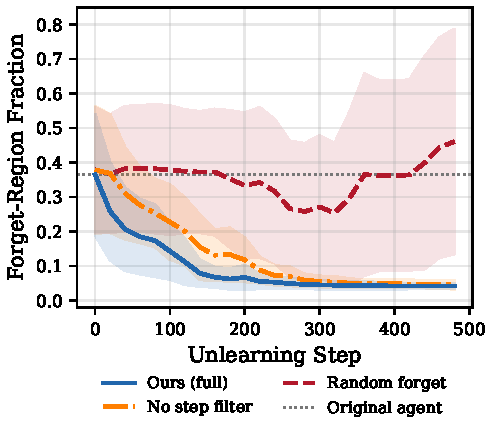
\includegraphics[width=0.8\columnwidth]{paper_figures/unlearning_curves.pdf}
  \caption{Forget-region fraction during unlearning. Our method (blue, solid) converges consistently across seeds; random forgetting (red, dashed) is unreliable. The gray dotted line shows the original agent's occupancy.}
  \Description{Line plot showing forget-region fraction decreasing steadily for our method but remaining inconsistent for random forgetting over 500 unlearning steps.}
  \label{fig:unlearning_curves}
\end{figure}

\subsection{Full Retraining Analysis}

Figure~\ref{fig:retrain_curves} illustrates the cost of full retraining: while it eventually matches our forget-region fraction, it requires 500{,}000 steps and returns plateau at 60, 80 (vs.\ our 500/500). The $-1$ penalty reshapes the reward landscape, forcing the agent to sacrifice episode length for spatial compliance. Our method (dashed blue lines) achieves both objectives in three orders of magnitude fewer updates.

\begin{figure}[t]
  \centering
  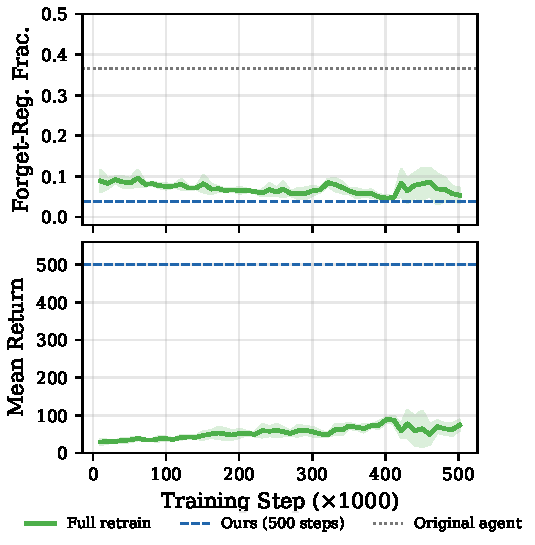
\includegraphics[width=0.75\columnwidth]{paper_figures/retrain_curves.pdf}
  \caption{Full retraining over 500k steps. Top: forget-region fraction converges slowly. Bottom: returns remain low (${\sim}$80) due to reward shaping. Dashed blue lines show our method's results achieved in just 500 steps.}
  \Description{Two-panel plot showing full retraining's forget-region fraction and return over 500k steps, with our method's results shown as horizontal reference lines.}
  \label{fig:retrain_curves}
\end{figure}

\subsection{Reliability Across Seeds}

Figure~\ref{fig:scatter} plots per-seed results in the forget-region fraction vs.\ return plane (ideal: upper-left). Our method (blue circles) and fine-tuning (purple crosses) both cluster in the ideal region, though our method clusters most tightly. Full retraining (green squares) achieves low forget-region fractions but at severely reduced returns. Random forgetting (red triangles) scatters widely, with one seed in the upper-left but another in the upper-right. Each baseline thus has a distinct failure mode: full retraining fails on \emph{retain stability}, random forgetting fails on \emph{forget effectiveness}, and fine-tuning clusters with our method but requires 100$\times$ more steps. Only targeted behavioral unlearning succeeds on both dimensions efficiently.

\begin{figure}[t]
  \centering
  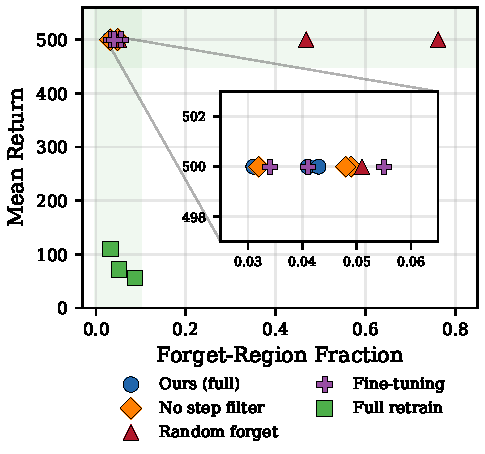
\includegraphics[width=0.8\columnwidth]{paper_figures/per_seed_scatter.pdf}
  \caption{Per-seed results in the forget-region fraction vs.\ return plane. The ideal region is the upper-left. Our method, no-step-filter ablation, and fine-tuning all cluster there; full retraining sacrifices return; random forgetting scatters unpredictably.}
  \Description{Scatter plot showing five methods across three seeds each, with our method tightly clustered in the ideal upper-left region.}
  \label{fig:scatter}
\end{figure}

%% ============================================================
\section{Discussion}

\paragraph{Positioning within RL unlearning.} Our baselines exhibit different failure modes than those in prior work. Ye et al.~\cite{ye2024reinforcementunlearning} find that retraining fails because representations generalize across environments; in our single-environment setting, retraining \emph{succeeds} at forgetting but at enormous cost and with severe performance degradation. Both works observe over-unlearning: our anchor term and low learning rate prevent policy collapse, analogous to their finding. Existing methods span a granularity spectrum, environment-level~\cite{ye2024reinforcementunlearning}, trajectory-level~\cite{gong2024trajdeleterenablingtrajectoryforgetting}, and our step-level approach, with finer granularity essential when the forget target is a continuous state-space property.

\paragraph{Behavioral vs.\ data-level unlearning.} Traditional unlearning removes specific \emph{data points}; behavioral unlearning removes \emph{behaviors}, state-action associations in a policy. The same trajectory may contain both desirable and undesirable behaviors, requiring step-level treatment. Our ablation quantifies this: omitting step-level filtering reduces the behavioral shift by 38\% (Table~\ref{tab:results}). This complements safe RL~\cite{garcia2015comprehensive}, which avoids unsafe states \emph{during} training; behavioral unlearning corrects them \emph{post-hoc} using only stored trajectories, without environment access.

\paragraph{Limitations.} While we evaluate on two environments with different forget criteria (spatial and orientation-based), both use discrete action spaces and relatively low-dimensional states. Real-world applications may involve continuous actions, high-dimensional observations, and more complex forget-region geometries. The method requires stored trajectories; agents deployed without trajectory logging would need alternative approaches. Our evaluation is limited to PPO; extending to other policy-gradient methods remains future work. Finally, we do not yet provide formal guarantees that forgotten behavior cannot be recovered through fine-tuning or adversarial probing.

\paragraph{Broader implications.} As RL agents are deployed in safety-critical domains, the ability to efficiently correct learned behaviors becomes essential. Behavioral unlearning offers a middle ground between full retraining (expensive, performance-degrading) and fine-tuning (requires environment access, unstable convergence). Figure~\ref{fig:bar} summarizes the trade-offs.

\begin{figure}[t]
  \centering
  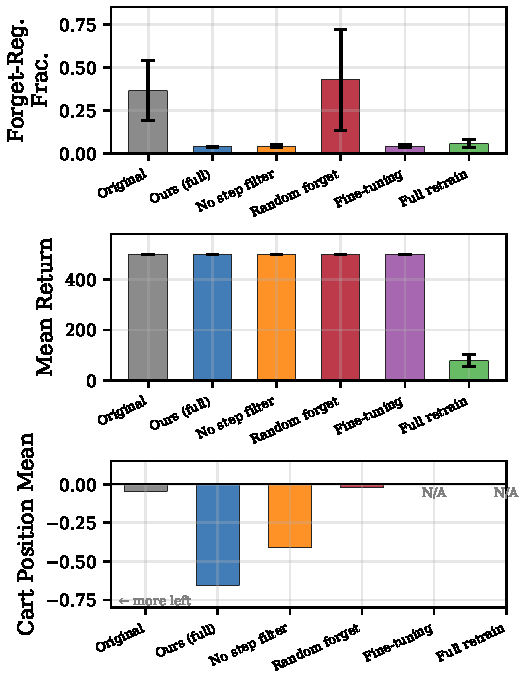
\includegraphics[width=0.7\columnwidth]{paper_figures/bar_comparison.pdf}
  \caption{CartPole summary: forget-region fraction (top), mean return (middle), and mean cart position (bottom). Our method achieves the best combination of all three metrics.}
  \Description{Three-panel bar chart comparing six methods on forget-region fraction, mean return, and cart position mean.}
  \label{fig:bar}
\end{figure}

%% ============================================================
\section{Future Work}
%% ============================================================
\balance

Several directions remain open. First, scaling to \textbf{continuous-control tasks} (e.g., MuJoCo) and high-dimensional observation spaces will test whether step-level filtering generalizes to richer domains. Second, providing \textbf{formal unlearning guarantees}, analogous to $(\epsilon, \delta)$-approximate unlearning in supervised learning~\cite{ginart2019makingaiforgetyou}, would strengthen applicability in regulated domains. Third, investigating \textbf{robustness to recovery attacks}: can an adversary recover the forgotten behavior through fine-tuning? Finally, combining behavioral unlearning with \textbf{continual learning safeguards} could enable agents that both acquire and selectively forget skills in a unified framework.

%% ============================================================
\section{Conclusion}
%% ============================================================

We introduced targeted behavioral unlearning for on-policy RL agents, a method that selectively removes behaviors associated with specific regions of the state space. Our trajectory-selective approach with step-level filtering achieves comparable forget effectiveness in two to three orders of magnitude fewer gradient updates than fine-tuning or retraining baselines, while maintaining task performance, and demonstrates consistent, reliable forgetting where random trajectory selection fails.

Our ablation study reveals a two-level hierarchy of importance: (1)~\emph{which trajectories} to unlearn matters most, random selection produces unreliable and sometimes counterproductive results; (2)~\emph{which steps within those trajectories} to target provides further precision, improving the strength of the behavioral shift by 38\%. Together, these findings establish that behavioral unlearning in RL requires careful, granular targeting at both the trajectory and transition level.

These results, validated across two environments with different forget criteria (position-based and orientation-based), position behavioral unlearning as a distinct and practically important problem in RL, complementary to existing environment-level~\cite{ye2024reinforcementunlearning} and trajectory-level~\cite{gong2024trajdeleterenablingtrajectoryforgetting} approaches, and orthogonal to continual learning methods that protect against accidental forgetting~\cite{kirkpatrick2017overcoming}.

\begin{acks}
Supported by the EKÖP-25 University Research Scholarship Program of the Ministry for Culture and Innovation from the source of the National Research, Development and Innovation Fund.
\end{acks}

%% ============================================================
%% References
%% ============================================================

\bibliographystyle{ACM-Reference-Format}
\bibliography{introb2026}

\end{document}
